\documentclass[11pt]{ujarticle} %%uplatexを用いる際はこちらを使用
\usepackage{funinfosys}
\usepackage{url}
\usepackage[dvipdfmx]{graphicx}
%\usepackage[top=10truemm,bottom=20truemm,left=15truemm,right=15truemm]{geometry}
%\usepackage[backend=biber,style=ieee]{biblatex}
\usepackage{caption}
%\addbibresource{./mid_rep.bib}
\author{
b1017197 瀧本恒平\\指導教員 : 松原克弥
}
\course{Intelligent Systems Course} %% 知能システムコースの場合はこちらを使用
\title{ロボット制御システムにおけるOSS機能モジュール向け\\サンドボックスの実現}
\etitle{Implementation of a Sandbox for an OSS Function Module in Robot Control Systems}
\eauthor{Kouhei Takimoto}
\abstract{Open Source Software(OSS)ノードを組み合わせることによるロボットアプリケーション開発が一般化している.Robot Operating System(ROS) は,ロボットアプリケーション開発用のフレームワークであり,ロボット開発に必要な基本的な機能を,膨大な数の OSSノードとして提供している.これらの既存のノードを利用することで,ロボットアプリケーションの開発速度や品質が向上する.一方,OSSノードが消費する各計算資源量は,あらかじめ不明な場合が多い.消費資源量が明らかでないノードをシステムに組み込むことで,それらがシステムに想定外の負荷を与える可能性がある.本研究では,OSSノードの消費資源量を事前に見積もり,ノードが消費可能な計算資源量に適切な上限を設けることで,OSSノードのサンドボックスを実現する.これにより,OSSノードによる開発効率向上と,ロボット制御システムの安定性の両立を目指す.}
\keywords{ROS, OSS, サンドボックス}
\eabstract{Robotic application development by combining Open Source Software (OSS) nodes is becoming more common. The Robot Operating System (ROS) is a framework for developing robot applications and provides the basic functions necessary for robot development many OSS nodes. By using these existing nodes, the development speed and quality of robot applications can be improved. On the other hand, the amount of computational resources consumed by each OSS node is often unknown in advance. The inclusion of nodes whose resource consumption is not known may cause unexpected load on the system. In this study, we estimate the amount of resources consumed by OSS nodes in advance and set an appropriate upper limit to the amount of computational resources that can be consumed by the nodes to achieve a sandbox of OSS nodes. This will improve both the development efficiency of OSS nodes and the stability of the robot control system.}
\ekeywords{ROS, OSS, sandbox}
\begin{document}
\maketitle
%\vspace*{-.5cm}

\section{背景}
近年,様々な分野においてロボットの活用が拡がっている\cite{Pepper}\cite{RoBoHoN}.このロボットアプリケーション開発において,ROSを用いる機会が増えている.ROSとは,ロボット開発を効率化するアプリケーションフレームワークのことであり,ノードを複数組み合わせることでシステムを構築する.図\ref{fig:nodeExp}は,ノードを組み合わせることで構築したロボットアプリケーションの例である.このように,ノードはロボットを構成する1つの機能であり,ノード間通信によってデータを送受信することによりロボットの動作を決定する.図では,カメラ制御ノードが撮影したデータを画像処理ノードにより解析し,解析された画像データを受け取った経路決定ノードが,画像からロボットの移動経路を計算し,その移動経路データを受け取った移動制御ノードがロボットに移動を開始する命令を送ることでロボットが動作を開始するようになっている.図の画像処理ノードのように,様々なロボットに必要な共通の機能(画像処理\cite{ROSexample},顔検出\cite{facedetector}など)は,ROSのコミュニティによってOSSのノードとして提供されている.そのため,フルスクラッチで機能を実装していた従来のロボット開発に比べて,OSSノードを用いた開発は効率的であることから,ROSは現在のロボットアプリケーション開発において重要なフレームワークのひとつとなっている.
%ROS 2を研究対象とする理由(省略可能?)
% ROSには,ROS 1とROS 2の2種類が存在している.先にリリースされたROS 1では,TCPROSというROS独自のノード間通信を行うためのプロトコルを用意している.このROS 1でのノード間通信を開始する前に,ROSマスターという通信相手を問い合わせるためのパラメータサーバを起動しておくことが必要になる.そのため,ROSマスターに問題が起きた場合,ノード同士でのデータのやり取りが出来なくなるため,ロボットアプリケーション全体の動作が不安定になってしまうという問題がある.また,ROS 1がサポートしているOSもUbuntuのみであるという制約も存在した.ROS 2では,ROS 1で抱えていた問題点や制約を解消するために,通信プロトコルなどのアーキテクチャが大きく変更されている.そのため,一部のノードに問題が起きて停止した場合でも,ロボットアプリケーション自体は停止せず,ノードが復帰すると正常に動くようになる.
%また,ROSには,ROS 1とROS 2の2種類が存在している.
% 先にリリースされたROS 1では,サポートOSはUbuntuのみであったが,ROS 2では,Ubuntuに加えWindowsやOS Xをサポートしている.また,ブリッジと呼ばれるROS 2のパッケージを用いることで,開発途中のROS 2においてもROS 1で開発されていた膨大なソフトウェア資産を使用できるようになるため,今後はROS 2の利用拡大が予想される.そのため,本研究ではROS 2を対象とする.
本研究では,ROSの次世代バージョンであるROS 2を対象として実装を行う.

\begin{figure}[t]
   \centering
   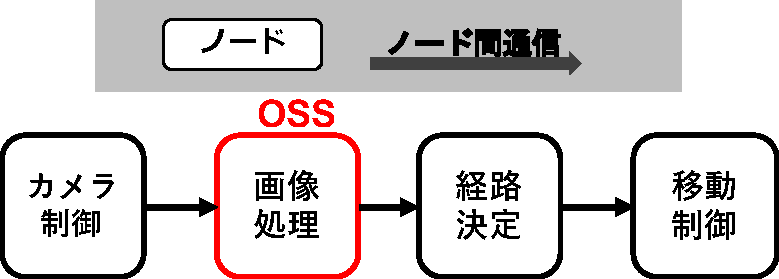
\includegraphics[width=7cm]{img/nodeExp.pdf}
   \caption{ノードを用いたシステムの例}
   \label{fig:nodeExp}
\end{figure}

\section{課題}
% ロボットの高機能化にともなって,ロボット制御システムにおける脆弱性の報告が増えている\cite{ROSSec}.これは,多種多様なOSSノードを再利用し,組み合わせることでシステムを構築するROSにおいて深刻な問題となる.
ROSでは,OSSノードの動作がシステム内の他のノードの動作に悪影響を与える可能性がある.その理由として,OSSノードのような第3者が作成したノードをシステムに組み込む際,開発効率を考慮すると,ノードの動作や計算資源消費量の詳細について確認することは少ないということがある.図\ref{fig:before}は,実際にOSSノードを取り入れたロボット制御システム(ドローン)の例であり,フルスクラッチで実装した移動制御ノード,位置情報取得ノードに加え,OSSである画像処理ノードを取り入れたシステムの一例である.ここでは,OSS画像処理ノードがシステム内の計算資源を専有してしまい,その影響を受けた移動制御ノードは必要分の計算資源を利用できない.そのため,ロボット制御システムの動作が不安定になっている.
% このように,ロボット制御システムで利用可能な計算資源の量には上限があるため,ROSでは,OSSノードのような第三者が作成した計算資源消費量の予測できないノードが,システム内の他のノードの動作に影響を与える可能性がある.
% 特に,デバイス上で共有利用している計算資源であるCPU,メモリ,ネットワーク帯域幅の消費量は,各ノードが必要とする計算資源消費量を事前に見積もることが難しい.加えて,現在のROSシステムでは,ノードごとの計算資源の管理を行うための機構が備わっていないため,ROSの分散環境におけるノードの割り当てが不均衡になり,計算資源を効率的に利用できない\cite{ResourceManeger}.

\begin{figure}[t]
   \centering
   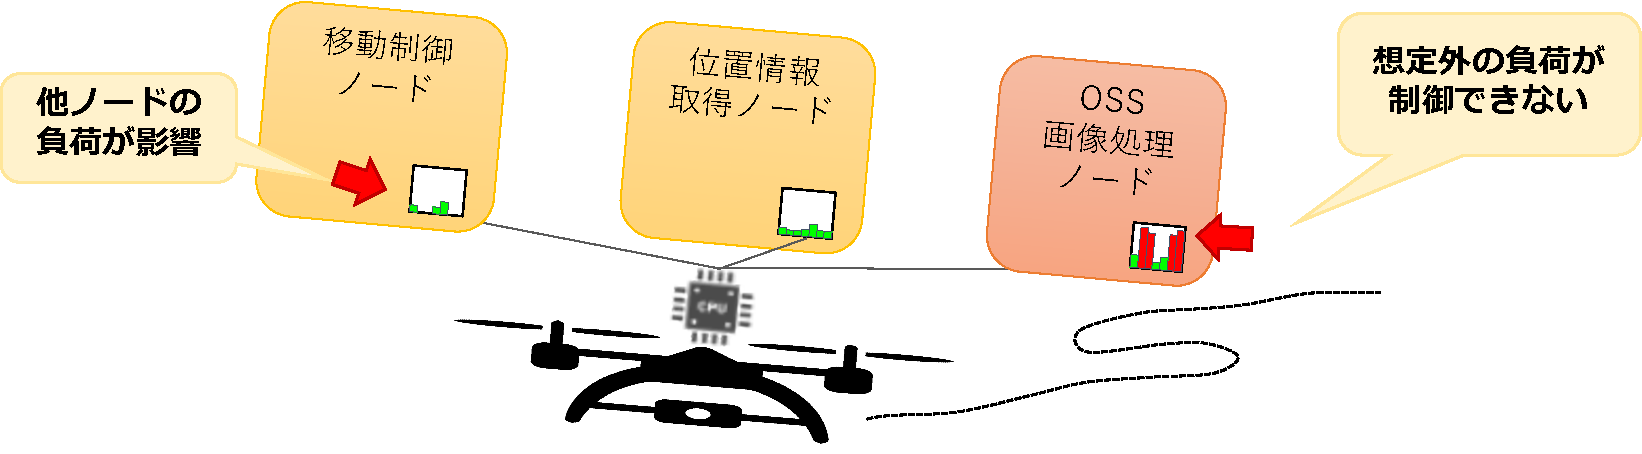
\includegraphics[width=7cm]{img/before.pdf}
   \caption{ロボット制御システムの例}
   \label{fig:before}
\end{figure}
% \begin{center}図1 ロボット制御システムの例\end{center}

\section{提案する手法:サンドボックスの作成}
前章までで述べたとおり,ROSを用いたロボット制御システムの開発においてOSSノードを用いることには,同一システム内の他ノードの動作に悪影響を与える可能性があるという課題がある.本研究では,OSSノードによるシステムへの想定外の負荷を防ぐことを目的として,各ノードを対象としたサンドボックスの作成を提案する.ここでのサンドボックスとは計算資源の最大消費可能量に制限をかける機構のことを指す.
% \subsection{サンドボックス設定のフロー}

はじめに,サンドボックスを作成する前に,サンドボックス作成に必要な情報を得るため,シミュレータを用いてノードの計算資源消費量について見積もりを行う.次に,見積もり結果から,サンドボックスで制限する計算資源量の上限を設定し,各ノードに対応したサンドボックスを作成する.これにより,図\ref{fig:after}のようにOSS画像処理ノードの使用可能な計算資源量の上限がコントロールされ,移動制御ノードは必要とする分の計算資源を使用できる.そのため,不安定であったロボット制御システムの動作が安定するようになると考えることができる.

\begin{figure}[t]
   \centering
   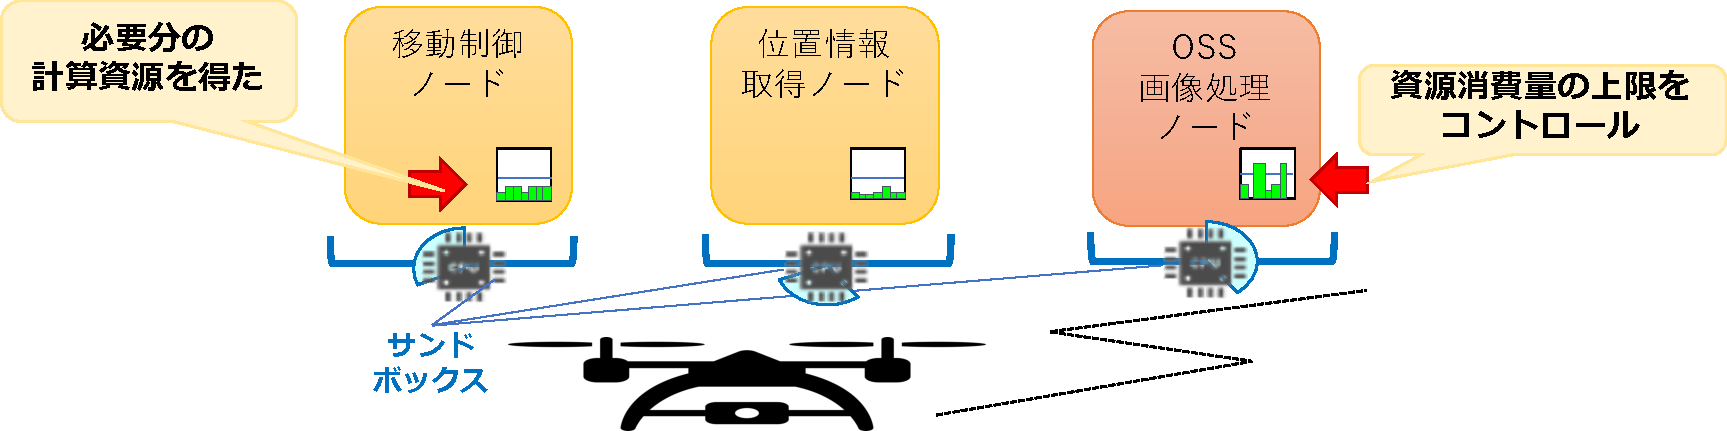
\includegraphics[width=7cm]{img/after.pdf}
   \caption{サンドボックス導入後のロボット制御システムの例}
   \label{fig:after}
\end{figure}

\subsection{今後の課題}
今後の課題として,ノードの計算資源消費量の見積もり手法の具体化がある.シミュレータ上でシステムをどれほどの時間動作させれば,求めている計算資源消費量やノードの動作の詳細を得ることができるのかについて検討する必要がある.また,シュミレータ上でシステムを動作させることで得ることができる計算資源消費量の記録から,システム全体の動作に悪影響を及ぼさず,ノードが最低限動作するような計算資源量を導出し,それをもとにサンドボックスの設定を行う必要がある.今後はノードの計算資源消費量の記録をもとに見積もりを行うための基準について検討していく.

\section{実現手法}
\subsection{手順 1:ノードの計算資源消費量見積もり手法}
はじめに,ロボットを実環境で動作させる前に,サンドボックスがどの計算資源をどれほどの数値に制限するかについて決定する.そのために,各ノードが消費するおおよその計算資源量を見積もる必要がある.この見積もりは,Gazebo\cite{Gazebo}によってロボットを仮想環境で動作させることで行う.Gazeboとは,ROSで一般的に用いるオープンソースの3Dロボットシミュレータである.これにより,各ノードを擬似的に動作させ,その動作中の各計算資源量を一定間隔で計測・記録する.この記録をもとに各ノードが消費する計算資源量の見積もりを行う.この計算資源消費量の計測には,Linuxのprocfsと,帯域幅監視ツールの一つであるNetHogsを使用する.procfsとは,Linuxからプロセス情報を取得するための仕組みである\cite{procMan}.また,NetHogsは,プロセスごとのトラフィック量を取得するものであり,ここではネットワーク帯域幅の取得に使用する.

\subsection{手順 2:Linux機能によるノードの計算資源消費量制限}
本研究におけるサンドボックスは,cgroupとtcコマンドによって各ノードの消費可能な計算資源量に上限を設定することで作成する.cgroupとは,ROSの動作プラットフォームであるLinux上で動作するコンテナ型仮想化環境を実現する機能の一つであり,プロセスの計算資源の利用を制限するLinuxカーネルの機能である\cite{cgroupMan}.cgroupには,旧バージョンのcgroup v1とその改良版のcgroup v2が存在する.cgroup v1では設定した計算資源量の上限を超過するとプロセスが停止してしまうが,cgroup v2であればプロセスを停止させずに計算資源消費量を抑えることができる.そのため,本研究では主にcgroup v2を使用する.しかし,cgroup v2は比較的新しい機能であるため,cgroup v1で使用されていた機能全てを使えるわけではない.そのため,cgroup v1とv2を共存させる形で使用する.cgroupの操作には,基本的にcgroupfsという擬似的なファイルシステムを用いる.新たにcgroupを作成する際も,通常のファイルシステムを扱うようにmkdirコマンドを用いることが可能である.

具体的にcgroupを用いてノードの計算資源消費量の制限を行うには,はじめにsys/fs/cgroup以下にcgroupを作成し,ノードのPIDをsys/fs/\\cgroup/cgroup.procsに登録する.その後,計算資源消費量の上限値をsys/fs/cgroup/cpu.max等に書き込むことで,CPU使用率とメモリ使用率の制限を完了できる.また,tcコマンドは,作成したネットワークインターフェースに対してネットワーク帯域制限を設定する機能である.ネットワーク帯域幅の制限についても,cgroupのnet\_clsを用いて,パラメータとネットワークインタフェースを設定することで制限を完了できる.

これらの設定を行うことで,本研究におけるサンドボックスを作成する.

\section{関連技術}
% 本研究の関連技術として,一般にコンテナ型仮想化技術と呼ばれる,アプリケーションコンテナがある.アプリケーションコンテナとは,アプリケーションを動作させるのに必要な環境を1つにまとめ,個別のサーバのように扱うことができるようにしたものである.このアプリケーションコンテナの一例として,Docker\cite{Docker}が存在する.アプリケーションコンテナは,Linuxカーネルの機能であるcgroupとnamespaceを用いて計算資源の制限と分離が可能であることに加え,コンテナの実行に必要な仮想環境の共有が容易であるなど,多くの機能を持つ.しかし,本研究で作成するサンドボックスが必要とする機能は計算資源消費量の制限のみである.そのため,本研究では実装の容易さや構造の簡略化を考慮してcgroupとtcコマンドを用いて,ノードの計算資源消費量の制御に特化したサンドボックスを作成する.
本研究の関連技術として,Dockerがある.Dockerとは,コンテナ型仮想化を用いてアプリケーションを実行するためのソフトウェアである.コンテナ型仮想化とは,アプリケーションの利用可能な計算資源を制限・隔離することで,仮想的な環境を低コストで実現する技術である.コンテナ型仮想化により,異なるマシン上でもアプリケーションの実行環境を統一し,消費計算資源量を制限できる.Dockerは,計算資源の制限と隔離にcgroupを用いるという点で,本研究の手法と関係性が深い.一方,Dockerには,仮想環境を配布する機能や,複数の仮想環境を管理する機能など,本研究とは関係のない機能が多数含まれている.したがって,本研究では,実装の容易さを考慮し,cgroupとtcコマンドを用いて,計算資源消費量の制限を行うこととした.

Fukutomiらは,ROS分散環境においてノードを動作させるホストマシン上の計算資源を効率的に利用するための計算資源管理機構を提案した\cite{ResourceManeger}.この研究では,計算資源使用率が一定に達したノードを動的に他のホストマシンに移行することで,分散環境上でも効率的にノードを動作させることを可能としている.本研究とはノードの計算資源消費量を制限せずにノードの動的移行を行うという点で異なっている.Fukutomiらの実現手法は,事前にノードの消費する計算資源量を把握していなくても,ノードを動的に移行することにより,システムを短い処理時間で動作させることができるという利点がある.しかし,ノードの動的移行を行う際,ノードが保持しているデータのバックアップを取る必要があるため,システムの動作中にオーバーヘッドが発生する.そのため,本研究では事前にノードの計算資源消費量を見積もり,サンドボックスを作成することで,システム動作中のオーバーヘッドなしに効率的な計算資源の利用を可能としている.

\section{おわりに}
\subsection{まとめ}
本研究では,OSSノードによるシステムへの想定外の負荷を最小限に抑えることを目的として,各ノードの消費可能な計算資源量に上限を設定するサンドボックスの作成を提案した.具体的には,Gazeboシミュレータ上でノードを動作させ,Linuxのprocfsと帯域幅監視ツールの一つであるNetHogsを用いて計算資源消費量を記録し,これをもとに計算資源消費量の見積もりを行う.見積もり結果より,コンテナ型仮想化機構の一つであるcgroupsとtcコマンドを用いて,ノードごとのCPU,メモリ,ネットワーク帯域の各計算資源における最大消費量に対して制限を課すことでサンドボックス機構を実現する.
%また,計算資源消費量を計測する間隔についても検討が必要である.

\section{知能システムコースにおける本研究の位置づけ}
知能システムコースでは,知能に関する課題および人と人工物の新たな関係性を構成論的な手法で追究する観点から,人の知的能力や機能の解明,数理モデル化,実世界への実装に関する具体的な課題に取り組み,その結果の評価を通じて,新しい方法論や,学問領域を切り拓く能力を育むことをカリキュラムポリシーとして掲げている.

本研究では,ROSという実世界への実装を補助する技術における課題を構成論的な手法で追究している.
% 今後は実装を行い,サンドボックス導入前と導入後で各ノードの計算資源消費量がどう変化したか,またシステムの動作パフォーマンスがどう変化するかを評価する.

%\printbibliography[title=参考文献]

\begin{thebibliography}{99}
  \bibitem{Pepper}
  \begin{flushleft}
  SoftBank:特集 \textbar ロボット\textbar ソフトバンク,入手先\textless https://www.softbank.jp/robot/special/\textgreater(参照2020-10-30).
  \end{flushleft}
  \bibitem{RoBoHoN}
  \begin{flushleft}
    SHARP CORPORATION:ロボホン,入手先\textless https://robohon.com/co/introduction.php\textgreater(参照2020-10-30).
    \end{flushleft}
  \bibitem{ROSexample}
  \begin{flushleft}
    Patrick Mihelich,James Bowman:ros-perception/image\_common,入手先\textless https://github.com/ros-perception/image\_common\textgreater(参照2020-11-03).
  \end{flushleft}
  \bibitem{facedetector}
  \begin{flushleft}
    Caroline Pantofaru:ROS Index,入手先\textless https://index.ros.org/p/face\_detector/\textgreater(参照2020-11-04).
  \end{flushleft}
  % \bibitem{ROSSec}
  % \begin{flushleft}
  % DiLuoffo,V., Michalson,R.W. and Sunar,B.:Robot Operating System 2: The need for a holistic security approach to robotic architectures,Proc.IJARS 2018,pp.1-15,SAGE Journals(2018).
  % \end{flushleft}
  \bibitem{Gazebo}
  \begin{flushleft}
  2014 OpenSource Robotics Foundation:Gazebo,入手作\textless http://gazebosim.org/\textgreater(参照2020-11-04)
  \end{flushleft}
  % \bibitem{RobotSecure}
  % 齋藤慶太,森達哉:コンシュマー向けロボットの安全な運用に向けたセキュリティポリシー,コンピュータセキュリティシンポジウム2017論文集,Vol.2017,No.2,pp.1426-1433(2017).
  % \bibitem{AutoWare}
  % Computing Platforms Federated \\Laboratory:CPFL/Autoware\_Toolbox,\\入手先\textless https://github.com/CPFL/\\Autoware\_Toolbox\textgreater(参照2020-10-30).
  \bibitem{procMan}
  \begin{flushleft}
  Michael Kerrisk:proc(5)-Linux manual page,man7.org,入手先\textless https://man7.org/linux/man-pages/man5/proc.5.html\textgreater(参照2020-10-30).
  \end{flushleft}
  \bibitem{cgroupMan}
  \begin{flushleft}
  Michael Kerrisk:cgroups(7)-Linux manual page,man7.org,入手先\textless https://man7.org/linux/man-pages/man7/cgroups.7.html\textgreater(参照2020-10-30).
  \end{flushleft}
  \bibitem{Docker}
  \begin{flushleft}
  Docker Documentation\textbar Docker Documentation, 入手先\textless https://docs.docker.com/\textgreater(参照2020-11-01).\end{flushleft}
  \bibitem{ResourceManeger}
  \begin{flushleft}
  Fukutomi,D.,Azumi,T.,Kato,S.,et al.:Resource Manager for Scalable Performance in ROS Distributed Environments,Proc.DATE 2019,pp.1088-1093,IEEE(2019).
  \end{flushleft}

\end{thebibliography}
\end{document}
%
%
% EOF
